\chapter{Cibles de fonctionnement}

proximité
-couvrir le territoire
-métiers traditionnels

expertise
-support technologique
-expertise et innovation

assurer gestion contractuelle et le reporting

gérer les interventions
intervention forfaitaire (préventif et curatif standard)
intervention en bon de commande (curatif exceptionnel, amélioration installations, traitement obsolescence...)

identification des risque techniques/financiers/organisationnels

améliorer le cadre de vie
respecter l'environnement

accompagnement dans la conception, la réalisation, l'exploitation et la maintenance d'installations plus économes en énergie et plus respectueuse de l'environnement
suivi de spécif client
suivi des avancements
construction et validation du processus commun avec les clients

revue périodique de contrat/évolution périodique du contrat -> décision de renouveler ou non l'affaire sous sa forme initiale ou une autre
réclamations clients (écarts constatés par le lcient)
négociation client (offre définitive validé avec le client)

preuve du respect des engagements (bonne mise en oeuvre et adaption au besoin)

compte rendu d'état des lieux initial (soldes d'écarts si travaux en plus nécessaires)




\section{Processus Retour d'exéprience}

\begin{figure}[h!]
	\centering
	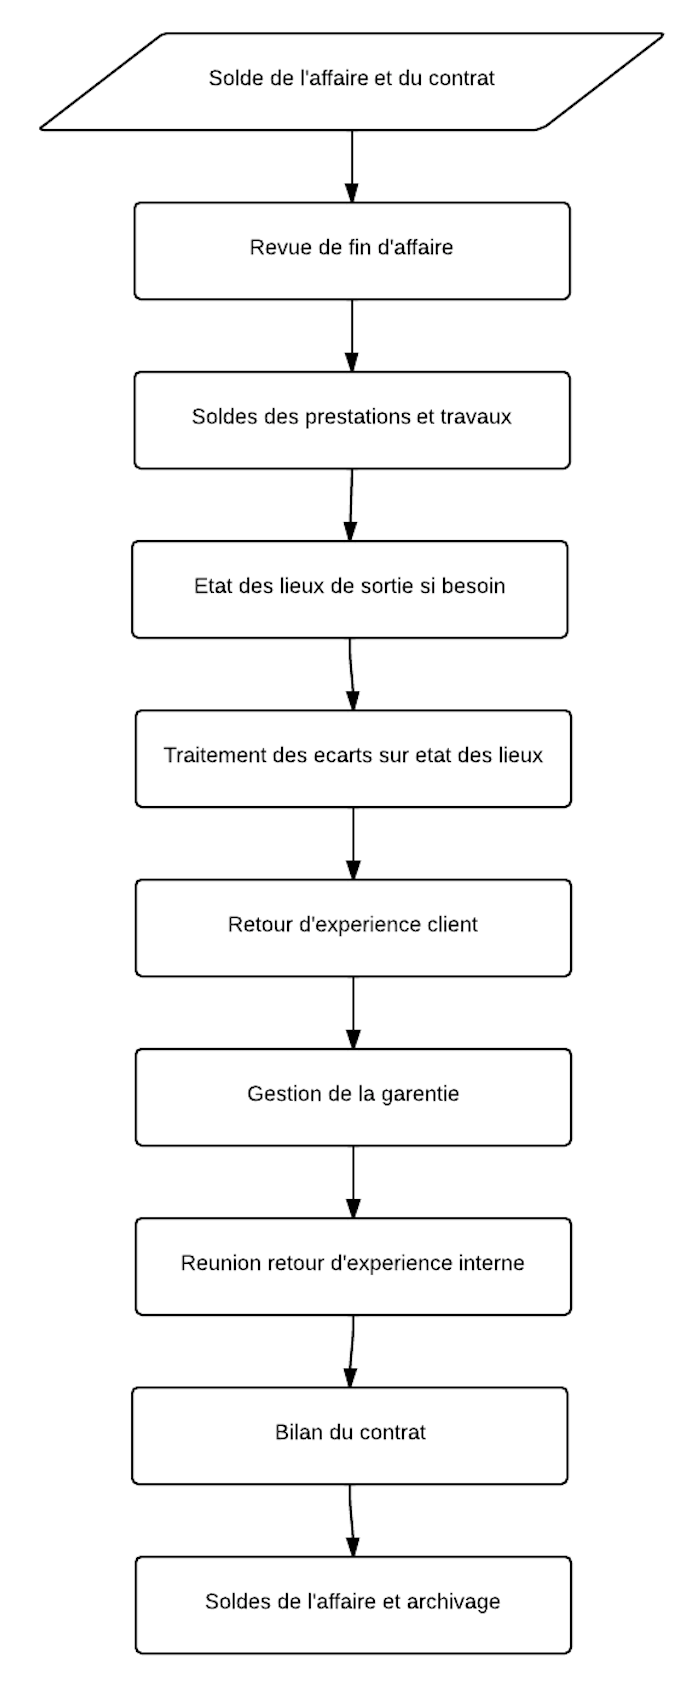
\includegraphics[width=0.45\linewidth]{images/processus_retour_experience.png}
	\caption{Processus de retour d'experience}
	\label{fig:processusRetourExperience}
\end{figure}

Ainsi l'ajout du processus \textit{retour d'\'exp\'erience client} dans le sous-processus \textit{solde
de l'affaire et du contrat} r\'epond aux exigences de SPIE Sud Est suivante~:

\begin{itemize}
    \item Base de connaissance m\'etier type de contrat~;
    \item Identification des risques techniques/financiers/organisationnels.
\end{itemize}

>>>>>>> 470c15da585d5cdfec473c9230a9522d360fd5b3
